\chapter{Introduction}
\label{chap-one}

Software implementation and maintenance are important parts of the software development process~\cite{krishnan2000empirical}. It is during these phases that developers complete actions to ensure quality software, such finding and resolving software defects and refactoring.
Many of the actions involved in writing and maintaining software are manual, tedious and, as a result, error-prone.
Tools, known as \textit{program analysis tools}, exist for developers to automate some of theses tasks and reduce the effort involved in tasks like defect finding and resolution~\cite{bruckhaus1996impact}. 
Some program analysis tools, known as static analysis tools, allow developers to find and resolve defects early in the development process and occasionally to find defects previously overlooked~\cite{ayewah2010google,Ayewah:2008:FindBugs}.

Research has found, however, that developers use these tools infrequently in practice~\cite{Ayewah:2008:FindBugs, ge2012reconciling, smith2015questions}. 
Multiple studies have explored developers' usage of program analysis tools and cumulatively found that developers encounter various challenges when attempting to understand and resolve problems in their code~\cite{johnson2013don,smith2015questions,christakis2016developers}. 

This dissertation proposes and evaluates the following:

\vspace{0.5em}

\noindent\fbox{\centering
	\parbox{\textwidth}{ \centering
	Program analysis \emph{tool use} is a form of \emph{communication} and \emph{inability to interpret and}\\ \textit{ resolve} notifications is a result of \emph{miscommunication} caused by \emph{knowledge gaps} and \\
	\emph{knowledge mismatches}; therefore we can improve tool design by providing the means for \\tools to \emph{classify} individual developer's \emph{conceptual knowledge} and adapt notifications  \\accordingly, leading to the potential for \emph{reducing time} required for developers to resolve \\tool notifications, \textit{increasing ability to resolve}, and \textit{decreasing attempts made when resolving.}}
	}

\vspace{1em}

To provide concrete motivation for this research, consider Valerie. Valerie is a hypothetical software developer at a start-up company. She primarily writes Java code, though she did not learn to program in Java, and uses the Eclipse Integrated Development Environment (IDE). In her spare time, she builds her knowledge of Java programming concepts by contributing to open source software and using tools that provide feedback about the code she writes. While modifying code in the Sun JDK source code repository, she contributes code that results in the notification shown in Figure~\ref{fig:eclipse}. She has experience using FindBugs, so she is familiar with some of the ways FindBugs communicates. For example, she knows that an orange bug icon indicates a \textit{scary} bug and that by clicking the bug icon she can gain access to more information about the bug.

\begin{figure}
	\centering
	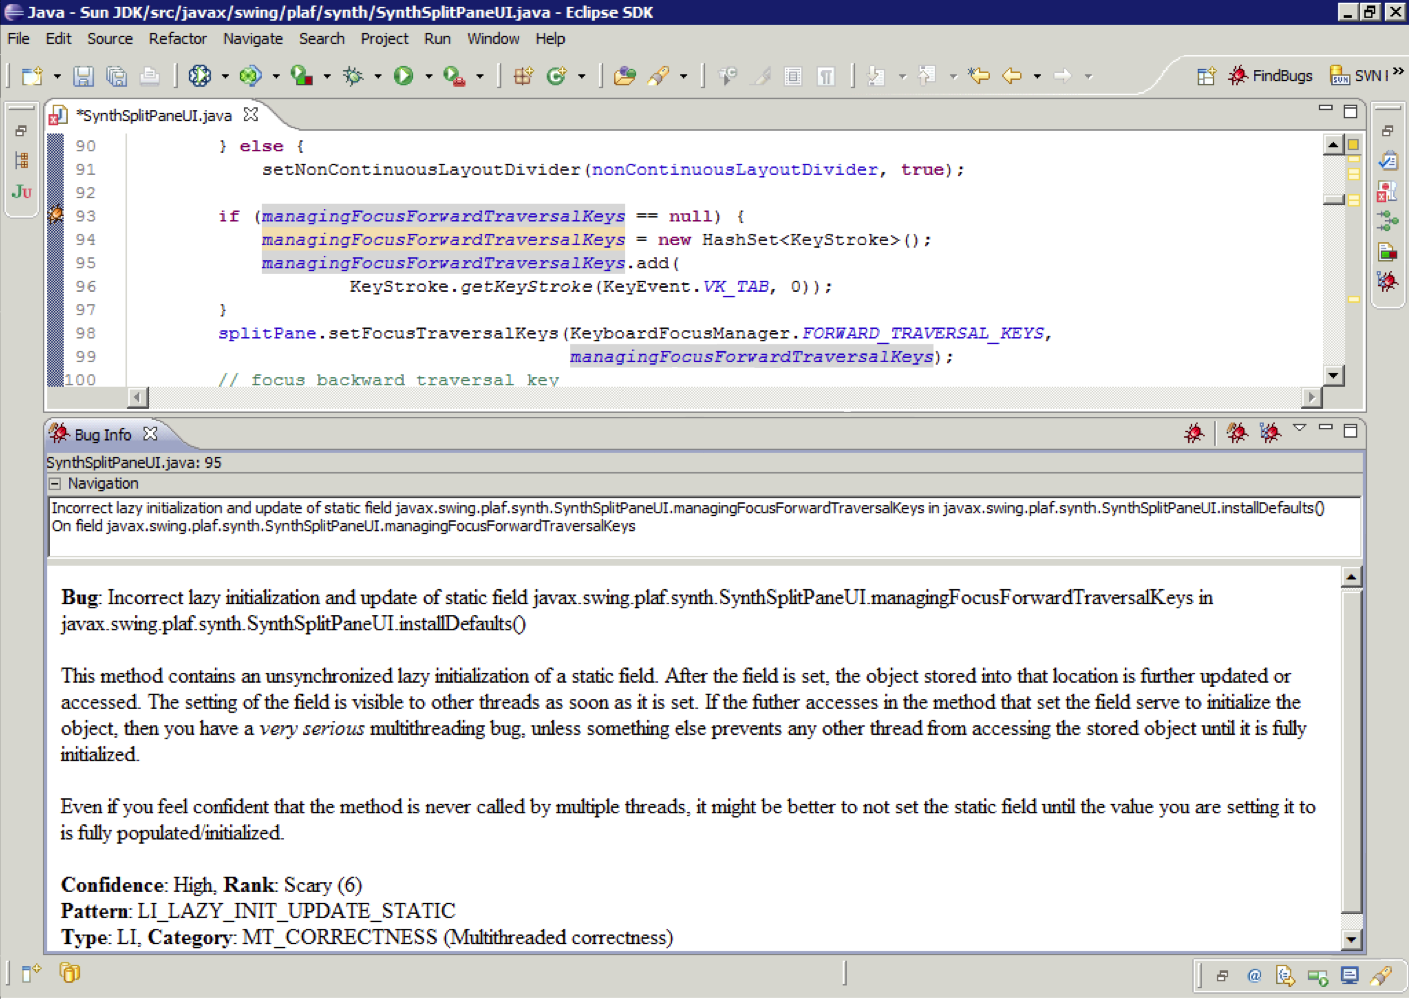
\includegraphics[width=\textwidth]{Chapter-2/figs/eclipse.png}
	\caption{Findbugs notification in the Eclipse IDE concerning multi-threading.}
	\label{fig:eclipse}
\end{figure} 

As she explores the information provided by FindBugs, she realizes that despite her experience with FindBugs, she is having difficulty determining how to resolve the notification. She first attempts to use what knowledge she does have regarding multi-threading, which she accrued from struggling with and resolving compiler synchronization warnings, to better understand the problem. 
% TODO not clear what "the problem" is - be specific
However, she is unfamiliar with the concept central to the notification in Figure~\ref{fig:eclipse} (lazy initialization). Though the notification tells her that the problem relates to multi-threading, she is unable to make a connection between her knowledge regarding multi-threading and the message FindBugs is attempting to communicate and therefore cannot resolve the notification without outside help. As done previously with compiler synchronization notifications, she toggles between the web and her IDE to understand and resolve the notification.

% TODO compiler synchronization notification??

\begin{figure} 
	\centering
	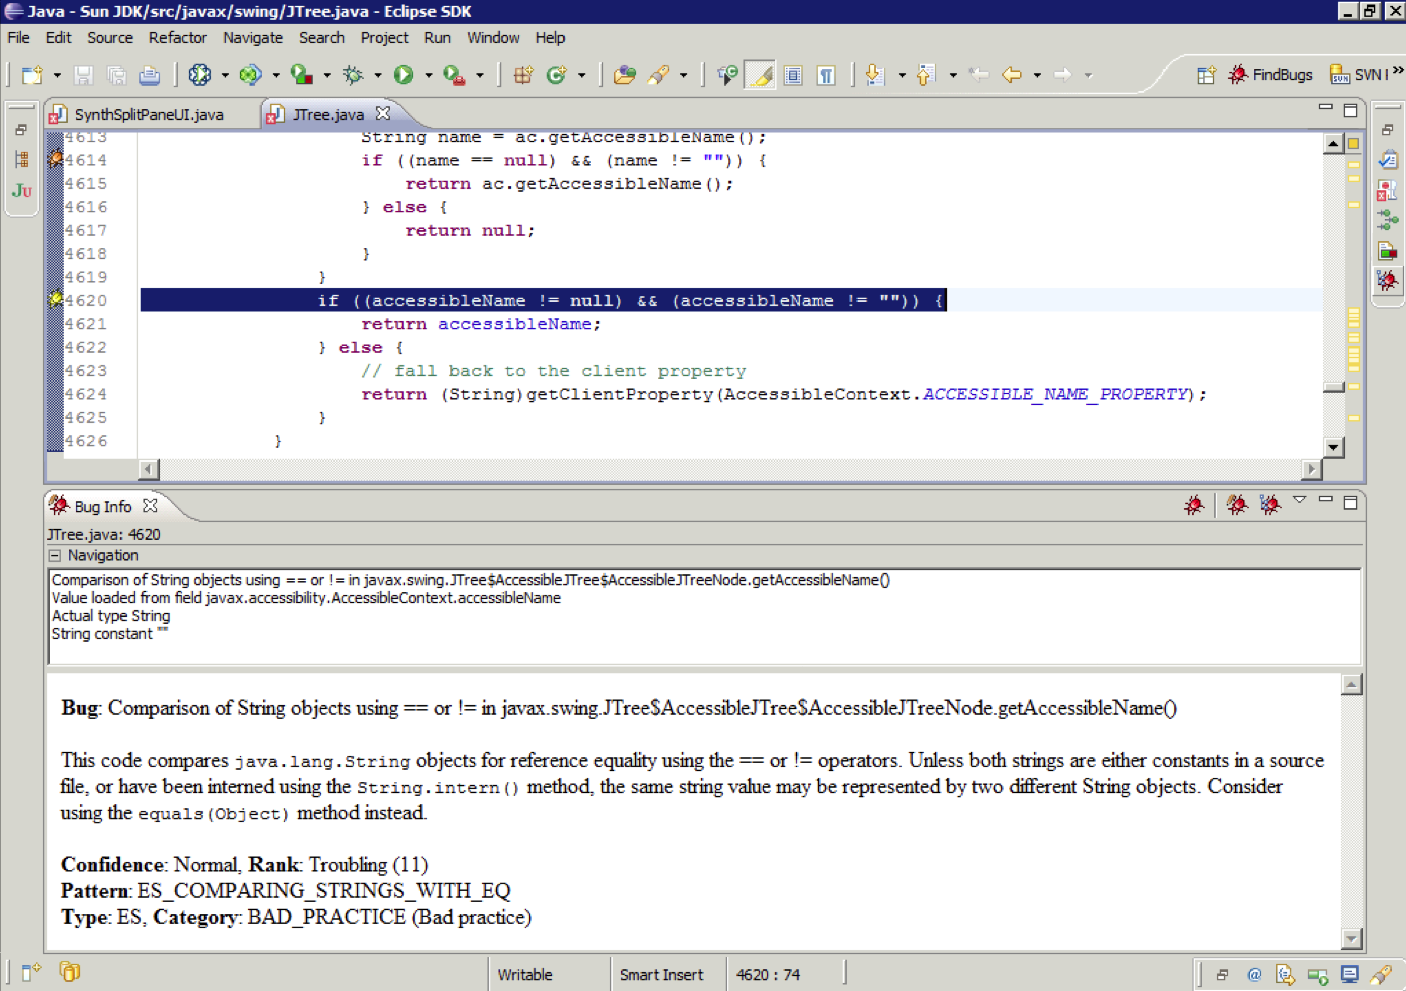
\includegraphics[width=\textwidth]{Chapter-2/figs/eclipse-2.png}
	\caption{Findbugs notification in the Eclipse IDE on checking string equality.}
	\label{fig:eclipse2}
\end{figure}

Although Valerie's goal when using tools like FindBugs is to find and resolve defects, which requires the ability to interpret the notifications provided by the tools, a secondary goal is to learn more about Java programming concepts. She found, however, that some notifications are better at communicating problems while contributing to knowledge than others. For example, when first learning how to work with strings in Java, Valerie encountered the notification in Figure~\ref{fig:eclipse2}. The first time she encountered the problem she was able to understand and resolve the notification. Looking back, she realizes this was because the notification in Figure~\ref{fig:eclipse2} filled in gaps in her own knowledge of the concept by informing her \emph{why} what she was doing was wrong and \emph{how} she can fix it.

Because the tools Valerie uses have no notion of what she does and does not know, some notifications communicate in a way that she is able to understand the problem, while others are not, leading to  miscommunication.
\textit{The goal of this research is to improve how program analysis tools communicate to developers by providing theories and approaches that identify and utilize the differences between developer information needs, based on their knowledge, that influence their ability to resolve tool notifications.}

In the following chapters, I will discuss the research I conducted to explore challenges like those encountered by Valerie and research for developing techniques, frameworks, and tools to mitigate these kinds of challenges.
Chapter~\ref{chap:rw} ground my research in existing research in Computer Science and other fields.
Study 1, outlined in Chapter~\ref{chap:why}, answers the following research questions:
\begin{itemize}
    \item [RQ\textsubscript{1}]: \textit{What reasons do developers have for using or not using static analysis tools to find bugs?}
    \item [RQ\textsubscript{2}]: \textit{How well do current static analysis tools fit into the workflows of developers? We define a workflow as the steps a developer takes when writing, inspecting and modifying their code.}
    \item [RQ\textsubscript{3}]: \textit{What improvements do developers want to see being made to static analysis tools?}
\end{itemize}

Based on findings from Study 1, which identified tool notification understandability as a barrier to use, Chapter~\ref{chap:theory} answers the research question \textit{why do developers encounter challenges when interpreting tool notifications?}.
I used the findings from Study 2 to formulate the boxed explanatory theory above regarding how knowledge affects developers' ability to interpret and resolve notifications.
Using this theory, Chapters~\ref{chap:assess} and~\ref{chap:experience} present Study 3, which answers the following research questions:
\begin{itemize}
    \item [RQ\textsubscript{1}]: \textit{Is source code a good predictor of how much developers know about programming concepts?}
	\item [RQ\textsubscript{2}]: \textit{Does concept-specific source code increase the ability to classify how much developers know about programming concepts in comparison to a naive model?}
\end{itemize}

In Chapter~\ref{chap:assess}, I outline an approach used to assess developer concept knowledge in preparation for the work done in Chapter~\ref{chap:experience} to predict developer concept knowledge.
Finally, based the ability to predict conceptual knowledge, I posit and evaluate the following hypotheses and research question in Chapter~\ref{chap:improve}:
\begin{itemize}
    \item [H\textsubscript{1}]: \textit{Knowledge-based notifications can decrease the time required for notification resolution.}
    \item [H\textsubscript{2}]: \textit{Knowledge-based notifications increase developer likelihood of resolving notifications. }
    \item [H\textsubscript{3}] Knowledge-based notifications decrease developer code churn when resolving notifications.
    \item[RQ]: \textit{Do developer adaptation preferences match expectations from existing problem solving literature?}
\end{itemize}

Findings from Study 4 suggest the possibility of improving developer ability to quickly resolve notifications. Though the differences observed in this study are small, it is a first step in the direction of better understanding how to improve tool use for developers. To conclude this dissertation, Chapter~\ref{chap:future} outlines possible directions for future work that builds the foundations set by this research in this thesis.

The contributions of this dissertation are as follows:
\begin{itemize}
    \item A categorized list of reasons developers have for not using program analysis tools, accompanied by tool design suggestions provided by developers.
    \item An explanatory theory for the challenges that developers encounter when interpreting information provided by tool notifications.
    \item An approach for assessing developer depth of programming concept knowledge that builds on an existing validated approach for assessing breadth of knowledge.
    \item An approach, developed using existing problem solving research, for adapting tool notifications based on developer concept knowledge.
\end{itemize}
